%==============================================================================
\documentclass[11pt,oneside,onecolumn,letterpaper]{article}
\usepackage{times}
\usepackage[paperwidth=8.5in, paperheight=11in,
top=2.5cm, bottom=2.6cm, left=2.58cm, right=2.53cm]{geometry}
%\setlength{\textheight} {9.00in}
%\setlength{\textwidth}  {6.40in}
%\setlength{\topmargin}  {-0.50in}
%%\setlength{\headheight} {0.00in}
%%\setlength{\headsep}     {0.40in}
%\setlength{\oddsidemargin}{-0.010in}
%\setlength{\evensidemargin}{-0.00in}
%==============================================================================
%\usepackage{algorithm}
\usepackage{amssymb}
\usepackage{color,soul}
\usepackage{booktabs}
\usepackage{graphicx}
\usepackage{latexsym}
\usepackage{subfigure}
\usepackage{wrapfig}
\usepackage{amsmath}
\usepackage{amsthm}
\usepackage[hyphens]{url}
\usepackage{pifont}
\usepackage{xcolor}
\usepackage{colortbl}
\usepackage{indentfirst}
\usepackage[lined, boxed, linesnumbered]{algorithm2e}
\usepackage[square, comma, sort&compress, numbers]{natbib}

\newcounter{alg}
\newenvironment{enum-ref}{
\begin{list}%
{[\arabic{alg}]} {\usecounter{alg}
  \setlength{\leftmargin} {0.25in}
  \setlength{\labelwidth} {0.30in}
  \setlength{\rightmargin}{0.00in}
  \setlength{\topsep}     {0.00in}}
}{\end{list}}

\newenvironment{enum-number}{
\begin{list}%
{\arabic{alg})} {\usecounter{alg}
  \setlength{\leftmargin} {0.25in}
  \setlength{\labelwidth} {0.30in}
  \setlength{\rightmargin}{0.00in}
  \setlength{\topsep}     {0.00in}}
}{\end{list}}

\newenvironment{enum-nonum}{
\begin{list}%
{$\bullet$} {
  \setlength{\leftmargin} {0.25in}
  \setlength{\labelwidth} {0.30in}
  \setlength{\rightmargin}{0.00in}
  \setlength{\topsep}     {0.00in}}
}{\end{list}}

\newcommand{\ziming}[1]{%
  \begingroup
  \definecolor{hlcolor}{RGB}{20, 255, 20}\sethlcolor{hlcolor}%
  \textcolor{black}{\hl{\textit{\textbf{Ziming:} #1}}}%
  \endgroup
}

\let\chapter\section

%==============================================================================
\pagestyle{plain}
%==============================================================================

\title{Protected Automotive Remote Entry Device (PARED) \\ System Design}
\author{MITRE eCTF 2023\\Team \textbf{Cacti}\\ University at Buffalo}
\date{}



\begin{document}
%%
%=============================================================================
\normalsize


\maketitle
%\date{}

\renewcommand{\thepage}{System Design, Team Cacti, University at Buffalo--\arabic{page}}
\setcounter{page}{1} \normalsize
%
%\renewcommand{\baselinestretch}{1.2}
%\normalsize
%\vspace{0.1in}
%\centerline{\textbf{\Large }}
%\renewcommand{\baselinestretch}{1.0}
%\normalsize

\newcommand{\flagRollback}{\textsf{Rollback}\xspace}

\section{Introduction}

This section presents the entities and communication channels in the system.

\subsection{Entities}

The following summarizes the entities in the system.

\section{Security Requirements}

This section defines the security requirements of our design.

\subsection{SR1}
\textbf{A car should only unlock and start when the user has an authentic fob that is paired with the car.}

In the reference design, ...

\paragraph{How we address it:} ...

\subsection{SR2}
\textbf{Revoking an attacker's physical access to a fob should also revoke their ability to unlock the associated car.}

In the reference design, ...

\paragraph{How we address it:} ...

\subsection{SR3}
\textbf{Observing the communications between a fob and a car while unlocking should not allow an attacker to unlock the car in the future.}

In the reference design, ...

\paragraph{How we address it:} ...

\subsection{SR4}
\textbf{Having an unpaired fob should not allow an attacker to unlock a car without a corresponding paired fob and pairing PIN.}

In the reference design, ...

\paragraph{How we address it:} ...

\subsection{SR5}
\textbf{A car owner should not be able to add new features to a fob that did not get packaged by the manufacturer.}

In the reference design, ...

\paragraph{How we address it:} ...

\subsection{SR6}
\textbf{Access to a feature packaged for one car should not allow an attacker to enable the same feature on another car.}

In the reference design, ...

\paragraph{How we address it:} ...



\section{Security Implementations}



\subsection{Build PARED System}

\subsubsection{Build Environment}

This step will build the docker image from the Dockerfile. We will list all the additional packages we used besides those are in the reference design.

\subsubsection{Build Tools}

\textit{The resulting host tools will be given to the other teams in the Attack Phase.}

Our host tools are written in Python, thus this step will simply copy all the tools in to the docker container.

\subsubsection{Build Deployment}

\textit{Attackers will NEVER be given access to the Host Secrets generated in this step.}

In our design, the Host Secrets contain two parts: the Global Secret and the Car Secrets, and they will be saved in the \textit{secrets} docker volume.

This step will generate the Global Secret, which is a deployment-wide secret shared across cars and/or fobs.
The Global Secret is a pair of asymmetric encryption keys which contains a private key and a public key.
The private key is used to package the feature and will never get loaded to any of the car/fob devices.
The public key is used to authenticate the packaged feature and will get loaded to the paired fob.

We generate the Global Secret randomly, to prevent the attacker from retrieving it through reverse engineering.

\subsubsection{Build Car, Paired Fob, and Unpaired Fob}

\textit{The plaintext firmware and EEPROM files produced in these steps are not given to attackers except for the car and paired fob of Car 0 that will not contain any flags.}

\textit{These build steps may read and modify the Host Secrets.}

To build the car binaries, a car ID will be supplied as a flag to the building tools. We will:
\begin{itemize}
	\item Check whether the car secret that corresponding to this car ID exists in the \textit{secrets} docker volume.
	\item If it not exists, we randomly generate one, and save it into the \textit{secrets} docker volume.
	\item This car secret will get loaded into the car EEPROM data. The car ID will be saved in the car firmware.
\end{itemize}

To build the paired fob binaries, a car ID (corresponding to this fob) and a fob pairing PIN will be supplied as a flag to the building tools. We will:
\begin{itemize}
	\item Retrieve the car secret which corresponding to this car ID from the \textit{secrets} docker volume.
	\item Retrieve the public key from the \textit{secrets} docker volume.
	\item Encrypt the fob pairing PIN with the car secret.
	\item Save the car secret and public key into the paired fob EEPROM data. Save the car ID and encrypted fob pairing PIN in the paired fob firmware.
\end{itemize}

To build the unpaired fob binaries, we will:
\begin{itemize}
	\item Retrieve the public key from the \textit{secrets} docker volume.
	\item Save the public key into the paired fob EEPROM data.
\end{itemize}

\subsection{Load Devices}

\textit{Teams will not be able to modify any part of this step.}

After building the system, the firmware and EEPROM contents are loaded onto the microcontrollers by the provided tools.

\subsection{Host Tools}

\subsubsection{Package Feature}

\textit{Attackers will be given access to the packaged feature produced in this step in many scenarios.}

The package feature host tool receives the car ID and the feature number as flags, and is able to read the host secrets.
\begin{itemize}
	\item Pack the the car ID, feature number and some control padding together.
	\item Encrypt the package using the private key.
\end{itemize}

The resulting packaged feature is encrypted by the private key.

\subsubsection{Pair Fob}

\textit{This tool will not have access to Host Secrets.}

The following describe the sequence of pairing an unpaired key fob. It requires the host tool, a paired fob device and an unpaired fob. The paired and unpaired fobs are connected to the host computer through the UART0, and also connect each other through the UART0. The host tool takes a pairing PIN as an argument, which needs to be the same pairing PIN as previous used to pair/build the paired fob.

\begin{figure}[!htbp]
	\begin{centering}
		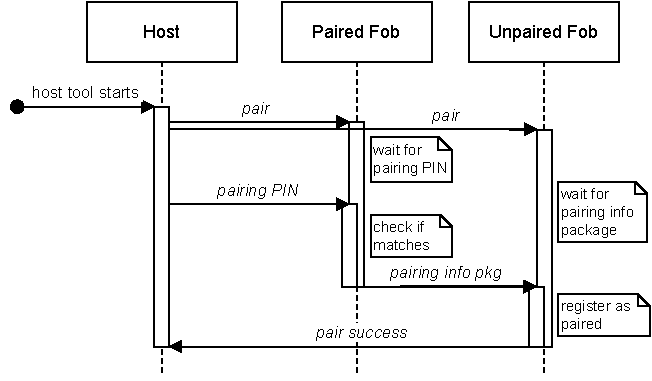
\includegraphics[width = .6\textwidth]{pic/pair.pdf}
		\caption{Pair Fob Sequence}
		\label{fig:pair}
	\end{centering}
\end{figure}

\begin{enumerate}
	\item The host tool starts the connection to both the paired and unpaired fob's UART0 sockets for serial transaction.
	\item The host tool sends the \textit{pair} command to both the paired and unpaired fob's sockets.
	\item After the paired fob receives the \textit{pair} command, it will enter the state to waiting for receiving the pair PIN from the same UART0 socket.
	\item After the unpaired fob receives the \textit{pair} command, it will enter the state to waiting for receiving the pairing info package from the UART1 socket which connects to the paired fob.
	\item The host tool sends the pairing PIN to the paired fob's UART0 socket.
	\item The paired fob receives the pairing PIN and encrypt it using the car secret. Then it checks the encryption result with the saved encrypted pairing PIN. If it matches, the paired fob will send the pairing info package to the UART1 socket. If it does not match, the paired fob will lockout for 3 seconds before resuming to listen to the UART messages.
	\item If the unpaired fob receives the pairing info package through the UART1 socket which connects to the paired fob, it will process the received package and use the info inside to register it as a paired fob.
	\item The unpaired fob (now it's paired) sends the pairing successful message to the UART0 to the host tool.
\end{enumerate}

Notes:
\begin{itemize}
	\item If the pairing PIN check in the paired fob fails, the paired fob will enter the lockout mode which blocks all the UART communication for 3 seconds. This is to prevent the brute force cracking of the pairing PIN.
	\item The pairing info package contains the car ID, the car secret and the encrypted pairing PIN.
\end{itemize}

\subsubsection{Enable Feature}

\textit{This tool will not have access to Host Secrets.}

The following describe the sequence of enabling a feature on a paired key fob. It requires the host tool, a paired fob device and the packaged feature. The paired fob is connected to the host computer through the UART0.

\begin{figure}[!htbp]
	\begin{centering}
		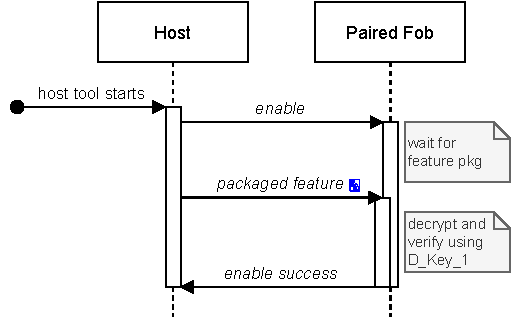
\includegraphics[width = .5\textwidth]{pic/enable.pdf}
		\caption{Enable Feature Sequence}
		\label{fig:enable}
	\end{centering}
\end{figure}

\begin{enumerate}
	\item The host tool starts the connection to the paired fob's UART0 sockets for serial transaction.
	\item The host tool sends the \textit{enable} command to the paired fob's socket.
	\item After the paired fob receives the \textit{enable} command, it will enter the state to waiting for receiving the packaged feature from the same UART0 socket.
	\item The host tool opens and sends the content of the packaged feature to the paired fob's socket.
	\item The paired fob receives and decrypts the package. If 1) the car ID in package matches the saved car ID, 2) the enabled feature list is not full, and 3) this feature has not been  enabled previously, the paired fob will enable this feature and save the new feature list.
	\item The paired fob sends the enable successful message to the UART0 to the host tool.
\end{enumerate}

Notes:
\begin{itemize}
	\item The paired fob uses the public key to decrypt the received package.
\end{itemize}

\subsubsection{Unlock and Start Car}

\textit{This tool will not have access to Host Secrets.}

The following describe the sequence of unlocking the car with a paired fob. It requires the host tool, a paired fob device and a car device. The car device is connected to the host computer through the UART0, and the paired fob connects to the car through the UART1. The connection between the car device and the host computer is only responsible for transmitting the messages that get printed out after the successful unlock.

\begin{figure}[!htbp]
	\begin{centering}
		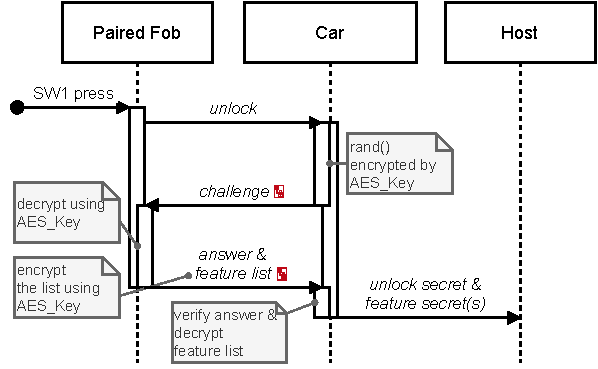
\includegraphics[width = .6\textwidth]{pic/unlock.pdf}
		\caption{Unlock Car Sequence}
		\label{fig:unlock}
	\end{centering}
\end{figure}

\begin{enumerate}
	\item The user press the SW1 button on the paired fob.
	\item The paired fob sends the \textit{unlock} command to the UART1 socket, and enter the state to waiting for receiving a respond from the same UART1 socket.
	\item After the car receives the \textit{unlock} command, it will generate a random number. Then this random number gets encrypted by the saved car secret. The result of this encryption is called \textit{challenge}.
	\item The car sends the \textit{challenge} package to the the UART1 socket, and enter the state to waiting for receiving a respond from the same UART1 socket.
	\item The paired fob receives the \textit{challenge} package and decrypt it using the saved car secret. The decrypted package (number) is called \textit{answer}. Then the paired fob sends this \textit{answer} package back to the UART1 socket.
	\item The car receives the \textit{answer} package and verify if it matches the previous generated random number. If it matches, the car will send the unlock message to the UART0 socket, and start the car (send the enabled feature list to the UART0 socket).
\end{enumerate}

\end{document}
%==============================================================================
